% =========================================================================== %
% Preamble                                                                    %
% =========================================================================== %

\documentclass[12pt, dvipsnames, aspectratio=169]{beamer}
%\documentclass[12pt, dipsnames, notes=only]{beamer}

\usepackage[utf8]{inputenc}
\usepackage{beamerthemesimple}

\date{December 8, 2020}
%\title{Access Control and Audit in the Appified IoT}
\title{BPFContain\footnote{If you have alternative name suggestions, let me know!}: Towards Secure and Usable Containers with eBPF}
\author{William Findlay}
\institute{Carleton University\\\href{mailto:will@ccsl.carleton.ca}{\ttfamily will@ccsl.carleton.ca}}

\usepackage{csquotes}
\usepackage{booktabs}

% Center floats by default
\makeatletter
\g@addto@macro\@floatboxreset{\centering}
\makeatother

\usepackage{listings}

\lstnewenvironment{listing}[1][]{\lstset{#1}}{}

\definecolor[named]{blue}{HTML}{0071b2}
\definecolor[named]{orange}{HTML}{e59c00}
\definecolor[named]{green}{HTML}{009e73}
\definecolor[named]{purple}{HTML}{88498f}
\definecolor[named]{dark-grey}{HTML}{515151}
\definecolor[named]{grey}{HTML}{797979}

\newcommand{\blue}[1]{{\color{blue}#1}}
\newcommand{\orange}[1]{{\color{orange}#1}}
\newcommand{\purple}[1]{{\color{purple}#1}}
\newcommand{\green}[1]{{\color{green}#1}}
\newcommand{\darkgrey}[1]{{\color{dark-grey}#1}}
\newcommand{\grey}[1]{{\color{grey}#1}}

\colorlet{listing-basic}{grey}
\colorlet{listing-keyword}{orange}
\colorlet{listing-keyword-2}{purple}
\colorlet{listing-keyword-3}{blue}
\colorlet{listing-comment}{green}
\colorlet{listing-string}{blue}

% Set default listings style
\lstdefinestyle{listingstyle}{
    basicstyle       = {\ttfamily\normalsize\color{listing-basic}\lst@ifdisplaystyle\footnotesize\fi},
    keywordstyle     = {\color{listing-keyword}\bfseries},
    keywordstyle     = {[2]\color{listing-keyword-2}\bfseries},
    keywordstyle     = {[3]\color{listing-keyword-3}\bfseries\itshape},
    sensitive        = true,
    commentstyle     = {\itshape\color{listing-comment}},
    stringstyle      = {\color{listing-string}},
    showstringspaces = false,
    literate = {~}{$\sim$}{1}
}
\lstset{style=listingstyle}

% yaml language for listings
\newcommand\YAMLkeystyle{\bfseries\color{listing-keyword-2}}
\newcommand\YAMLcolonstyle{\bfseries\color{listing-keyword-2}}
\newcommand\YAMLvaluestyle{\normalfont\ttfamily\color{listing-string}}
\lstdefinelanguage{yaml}{
  keywords={true,false,null,y,n},
  basicstyle = \YAMLkeystyle\ttfamily\normalsize\lst@ifdisplaystyle\footnotesize\fi,
  sensitive=false,
  comment=[l]{\#},
  morecomment=[s]{/*}{*/},
  stringstyle=\YAMLvaluestyle,
  moredelim=**[il][\YAMLcolonstyle{:}\YAMLvaluestyle]{:},   % switch to value style at :
  moredelim=**[l][\YAMLvaluestyle]{-},   % switch to value style at -
  morestring=[b]',
  morestring=[b]",
}

\setbeamertemplate{section in toc}[sections numbered]

\hypersetup{
    colorlinks = true,
    linkcolor  = .,
    urlcolor   = blue,
    citecolor  = blue,
}
\urlstyle{tt}

\newcommand{\fullframegraphic}[1]{%
    {%
        \usebackgroundtemplate{\includegraphics[width=\paperwidth]{#1}}
        \begin{frame}[plain]
        \end{frame}
    }
}

\newcommand\ufootnote[1]{%
    \begingroup
        \renewcommand\thefootnote{}\footnote{\hspace{-1.8em}#1}%
        \addtocounter{footnote}{-1}%
    \endgroup
}

% Table of Contents for sections
\AtBeginSection[]
{
    \begin{frame}[c, noframenumbering, plain]
        \begin{center}
        \Huge \bfseries \color{dark-grey} \insertsection
        \end{center}
    \end{frame}
}

\usepackage{biblatex}
\bibliography{../report/references.bib}
\setbeamertemplate{bibliography item}[text]

\usetikzlibrary{calc}

\usepackage{appendixnumberbeamer}

% =========================================================================== %
% Document                                                                    %
% =========================================================================== %

\begin{document}

% Optional watermark
\setwatermark[hoffset=6cm, voffset=0.3cm]{}

% Title page
\begin{frame}[noframenumbering, plain]
\titlepage
\begin{center}
\footnotesize COMP5900I Final Project Presentation
\end{center}
\end{frame}

\begin{frame}[c, noframenumbering, plain]{Outline of this Talk}
    \tableofcontents
\end{frame}

\section{Containers and Security}

\begin{frame}[c]{Containers vs Full Virtualization}
\begin{center}
  \color{black}
  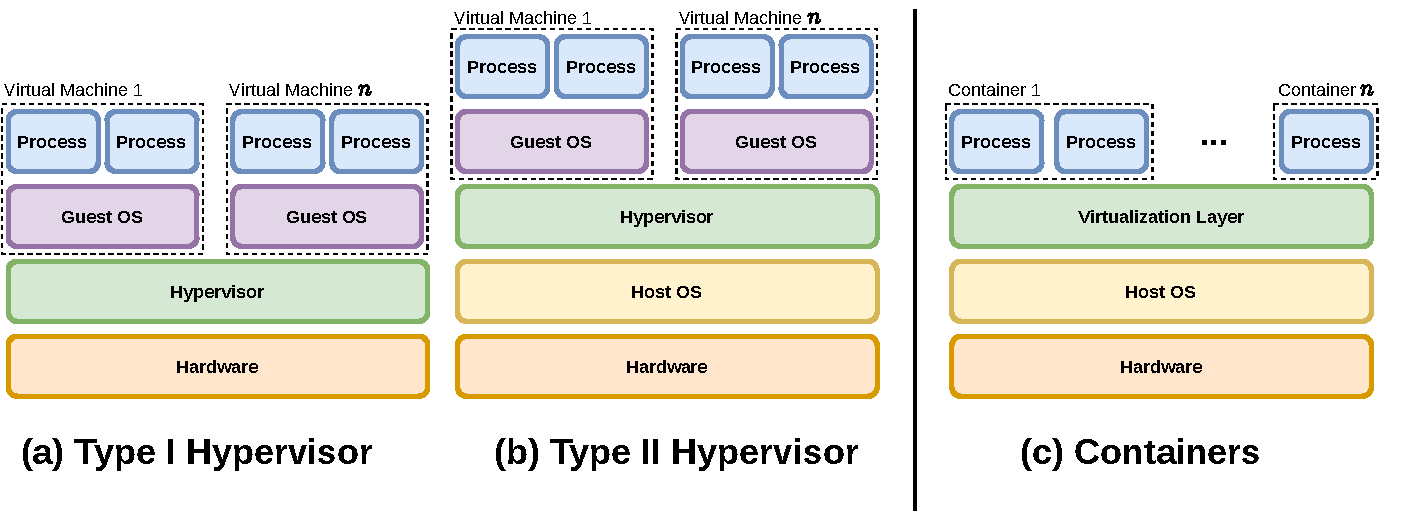
\includegraphics[width=0.9\textwidth]{figs/virtualization.pdf}
\end{center}
\ufootnote{Figure based on a simpler figure in \cite{sultan2019_container_security}}
\end{frame}

\begin{frame}[c]{Containers vs Full Virtualization}
\textbf{Containers:}
\begin{itemize}
  \item Lighter weight
  \item Share the underlying host OS kernel, resources
  \item Managed directly by the host OS
  \item Weaker isolation guarantees
\end{itemize}
\vfill
\textbf{Full Virtualization:}
\begin{itemize}
  \item Heavier weight (especially Type II)
  \item Each virtual machine includes its own guest operating system
  \item Managed by a hypervisor (sometimes without a host OS)
  \item Stronger isolation guarantees
\end{itemize}
\end{frame}

\begin{frame}[c]{Containers: Goals}
\textbf{\orange{Virtualization.}}
\begin{itemize}
  \item Give each container a \textit{virtual view} of system resources
  \item Process tree, filesystems, networking stack, memory, etc.
\end{itemize}
\vfill
\textbf{\blue{Least-Privilege.}}
\begin{itemize}
  \item \textit{Restrict access} to sensitive system resources
  \item Prevent a compromised container from compromising the rest of the system
\end{itemize}
\vfill
\textbf{\green{Composability.}}
\begin{itemize}
  \item Composable micro-services
  \item Allow containers to interact with each other (in pre-defined ways)
\end{itemize}
\ufootnote{Also dependency management, but we'll ignore that for now.}
\end{frame}

\begin{frame}[c]{Containers: Complexity}
\begin{columns}
  % Text column
  \begin{column}{0.5\textwidth}
    \orange{\bfseries Virtualization.}
    \begin{itemize}
      \item Filesystem mounts
      \item Namespaces
      \item Cgroups
    \end{itemize}
    \vspace{1.5em}
    \blue{\bfseries Least-privilege.}
    \begin{itemize}
      \item Unix DAC
      \item Seccomp
      \item POSIX capabilities
      \item MAC LSMs (e.g.~SELinux/AppArmor)
    \end{itemize}
  \end{column}
  % Graphics column
  \begin{column}{0.5\textwidth}
    \begin{center}
      \color{black}
      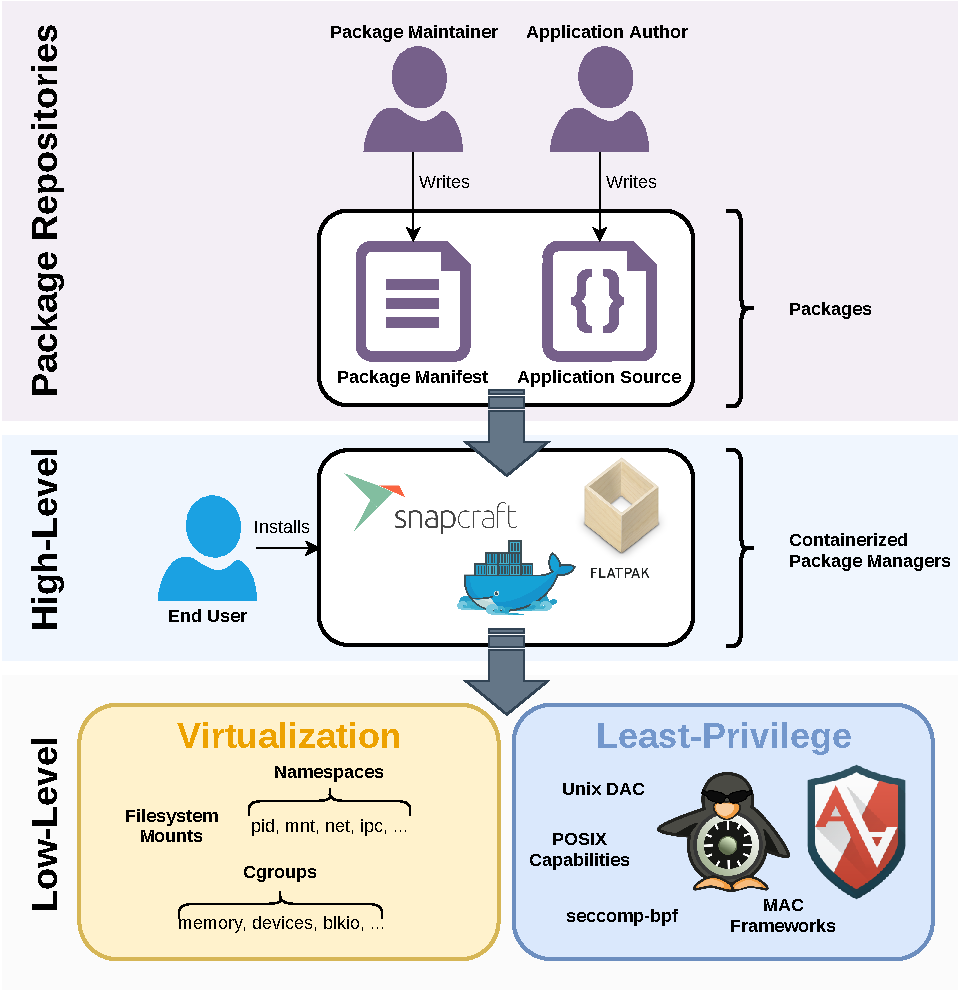
\includegraphics[height=0.8\textheight]{figs/containers.pdf}
    \end{center}
  \end{column}
\end{columns}
\end{frame}

\begin{frame}[c]{Containers: Security}
Container security is the \textbf{primary barrier} to widespread adoption \cite{sultan2019_container_security}.
\vfill
Container security is generally an \textbf{afterthought}.
\begin{itemize}
  \item Containers share the underlying OS kernel
  \item Proper virtualization/confinement requires elevated privileges (handle with care)
  \item Without \textbf{full} support for underlying security mechanisms
  (e.g.~MAC LSMs), we cannot achieve \blue{least-privilege}
\end{itemize}
\vfill
How can we \textbf{fix container security}?
\begin{itemize}
  \item Build containers to be \textbf{secure from the ground up}
  \item That means \textbf{start with \blue{least-privilege}}, make \orange{virtualization} optional
  \item Write an LSM \textbf{specifically for containers} \cite{sultan2019_container_security}
\end{itemize}
\end{frame}

\begin{frame}[c]{Containers: Threat Model}
\begin{center}
  \color{black}
  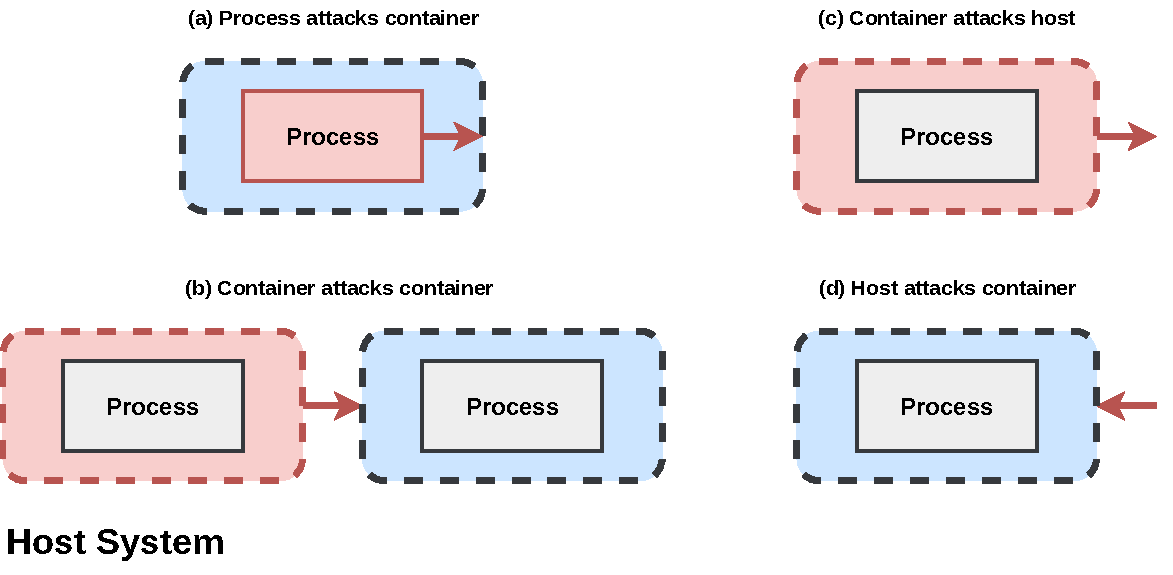
\includegraphics[height=0.7\textheight]{figs/threat-model.pdf}
\end{center}
\end{frame}

\begin{frame}[c]{Containers: Threat Model}
\begin{columns}
  \begin{column}[t]{0.4\textwidth}
    \textbf{Escalation of privilege.}
    \begin{itemize}
      \item Escape confinement
      \item Collusion attacks with other processes/containers
    \end{itemize}
    \vfill
  \end{column}
  \begin{column}[t]{0.4\textwidth}
    \textbf{Tampering.}
    \begin{itemize}
      \item Mess with other containers
      \item Mess with the host
    \end{itemize}
  \end{column}
\end{columns}
\vfill
\begin{columns}
  \begin{column}[t]{0.4\textwidth}
    \textbf{Information disclosure.}
    \begin{itemize}
      \item Reveal sensitive/secret information
    \end{itemize}
  \end{column}
  \begin{column}[t]{0.4\textwidth}
    \textbf{Denial of service.}
    \begin{itemize}
      \item Kill processes
      \item Disable interfaces
      \item Consume resources
    \end{itemize}
  \end{column}
\end{columns}
\end{frame}

\begin{frame}[c]{BPFContain's Mission Statement}
\begin{center}
\Huge
\textbf{Help defenders} by providing \textbf{simple, secure containers} with policy that is \textbf{easy to customize}.
\end{center}
\end{frame}

%\section{Containers in the Wild}
%
%\begin{frame}[c]{Docker}
%
%\ufootnote{Docker security documentation \cite{docker}}
%\end{frame}
%
%\begin{frame}[c]{Snapcraft}
%
%\end{frame}
%
%\begin{frame}[c]{Flatpak}
%
%\end{frame}
%
%\begin{frame}[c]{Container Problems}
%
%\end{frame}


\section{BPFContain Policy}

\begin{frame}[c]{Policy Design Goals}
\vfill
\begin{enumerate}
  \item Support the same basic functionality as Docker, Snap, etc.
  \begin{itemize}
    \item \blue{Confinement} + \orange{virtualization} (currently \blue{confinement} only)
    \item Have a way for containers to talk to each other (\green{composability})
  \end{itemize}
  \vfill
  \item Policy should be high-level, human-readable.
  \begin{itemize}
    \item Motto: \enquote{Be friendlier than bpfbox.}
  \end{itemize}
  \vfill
  \item No security knowledge required to read/write basic policy.
  \begin{itemize}
    \item If I want to stop behaviour $B_i$, I shouldn't \textbf{have to} tune $\{B_1,...,B_n\}$
    \item But, I should \textbf{be able to} if necessary
  \end{itemize}
  \vfill
  \item Least-privilege by default.
  \begin{itemize}
    \item Default-deny policy
    \item No need to \enquote{fall back to no security} like Docker, Snap, etc.
  \end{itemize}
\end{enumerate}
\vfill
\end{frame}

\begin{frame}[c]{Policy Language}
Policy language is written in YAML \cite{yaml}.
\begin{itemize}
  \item Simple, human-readable
\end{itemize}
\vfill
\textbf{Rights} and \textbf{restrictions}.
\begin{itemize}
  \item Rights $\equiv$ What the container is \textbf{allowed} to do.
  \item Restrictions $\equiv$ What the container is \textbf{not allowed} to do.
  \item A restriction \textit{always} overpowers a right.
\end{itemize}
\vfill
Policy is \textbf{default-deny}.
\begin{itemize}
  \item But you can use default-allow if you like
  \item Simple use cases, like blocking a specific feature
\end{itemize}
\end{frame}

\begin{frame}[c, fragile]{Example Policy: Discord}
Here's a policy that might be shipped with a Discord container:
\vfill
\begin{listing}[language=yaml]
name: discord
command: /usr/bin/discord
rights:
  - filesystem /
  - filesystem /proc readonly
  - network
  - video
  - sound
\end{listing}
\vfill
It fits on one slide!
\end{frame}

\begin{frame}[c, fragile]{Example Policy: Discord}
Suppose the user doesn't want Discord scanning \texttt{procfs}:
\vfill
\begin{listing}[language=yaml]
name: discord
command: /usr/bin/discord
rights:
  - filesystem /
  - network
  - video
  - sound
\end{listing}
\vfill
Just remove the access right!
\end{frame}

\begin{frame}[c, fragile]{Example Policy: Discord}
What if there is no existing policy? (And you don't want to write one)
\vfill
\begin{listing}[language=yaml]
name: discord
command: /usr/bin/discord
default: allow
restrictions:
  - filesystem /proc
\end{listing}
\vfill
Mark it as default-allow and specify a restriction.
\end{frame}

\section{BPFContain Implementation}

\begin{frame}[c]{BPFContain Components}
The \textbf{policy enforcement engine} is written in eBPF.
\begin{itemize}
  \item Maps contain per-container policy
  \item eBPF programs attached to LSM hooks enforce policy
  \item Another eBPF program attached to a special library call associates a process group
  with a container ID
\end{itemize}
\vfill
A \textbf{privileged userspace daemon} loads and manages BPF programs and maps.
\vfill
The user executes containers using an \textbf{unprivileged wrapper application}.
\begin{itemize}
  \item Launching a container requires \textbf{no additional privileges}
  \item You just run the container as an ordinary user
\end{itemize}
\end{frame}

%\begin{frame}[c]{Incremental Steps}
%\vfill
%\begin{enumerate}
%  \item The daemon loads BPF LSM programs and maps...
%  \vfill
%  \item Then it parses policy files...
%  \vfill
%  \item And populates maps with policy.
%  \vfill
%  \item The user launches container with bpfcon run.
%  \begin{itemize}
%    \item \texttt{\$ bpfcon run --name discord}
%  \end{itemize}
%  \vfill
%  \item bpfcon run invokes a special library call to start confinement...
%  \vfill
%  \item Then it runs the command associated with the container.
%\end{enumerate}
%\vfill
%\end{frame}

\begin{frame}[c]{BPFContain Architecture}
\begin{center}
  \color{black}
  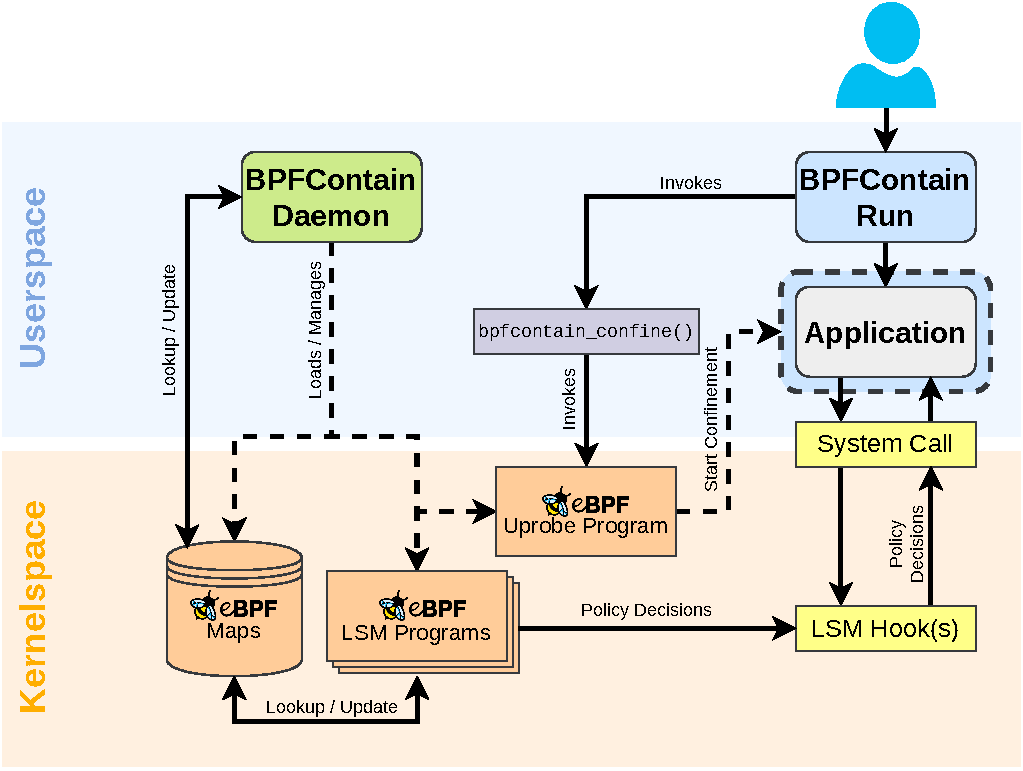
\includegraphics[height=0.85\textheight]{figs/architecture.pdf}
\end{center}
\end{frame}

\section{Conclusion}

\begin{frame}[c]{Future Work}
Add virtualization to policy language.
\begin{itemize}
  \item How to split things up?
  \item \texttt{mount} rules + \texttt{resource} rules?
  \item \texttt{namespace} rules + \texttt{cgroup} rules?
\end{itemize}
\vfill
New eBPF helpers for virtualization.
\begin{itemize}
  \item \texttt{bpf\_enter\_namespace()}
  \item \texttt{bpf\_enter\_cgroup()}
  \item \texttt{bpf\_remount()} (in mount namespace only?)
\end{itemize}
\vfill
\end{frame}

\begin{frame}[c]{Future Work}
%Add options for finer-grained confinement.
%\begin{itemize}
%  \item Something more bpfbox-like for advanced use cases?
%\end{itemize}
%\vfill
Get rid of the privileged daemon.
\begin{itemize}
  \item We don't need it (just pin the BPF maps/programs and exit)
  \item \texttt{\$ sudo bpfcon load-policy}
  \item \texttt{\$ sudo bpfcon logs}
\end{itemize}
\vfill
Global meta-policy.
\begin{itemize}
  \item A policy about what policy is allowed
  \item E.g.~\enquote{No default-allow policies on my system}
  \item E.g.~\enquote{No IPC between any containers}
\end{itemize}
\end{frame}

\begin{frame}[c]{Contributions}
BPFContain can be framed in different ways:
\begin{enumerate}
  \item A security-first approach to containers.
  \item A simple approach to confinement.
  \item A \enquote{container-specific} LSM implementation \cite{sultan2019_container_security}.
\end{enumerate}
\vfill
\begin{center}
BPFContain helps defenders by providing simple, secure containers\\and easily customizable policy.
\end{center}
\end{frame}

\appendix

\section{Backup Slides (eBPF 101)}

%\begin{frame}[c]{Programs and Maps}
%\textbf{Programs} are written in a restricted subset of C.
%\begin{itemize}
%  \item Compiled into BPF bytecode
%  \item Loaded into the kernel and attached to events with \texttt{bpf(2)}
%  \item JIT compiled into native instruction set
%\end{itemize}
%\vfill
%\textbf{Maps} are specialized key-value data structures for storing event data.
%\begin{itemize}
%  \item Created in the kernel using \texttt{bpf(2)}
%  \item May be accessed directly by eBPF programs
%  \item May be accessed from userspace with \texttt{bpf(2)} or \texttt{mmap(2)}
%\end{itemize}
%\end{frame}

\begin{frame}[c]{eBPF In a Nutshell}
%eBPF provides \textbf{safe kernel extension} and \textbf{system observability}.
%\vfill
\begin{center}
  \color{black}
  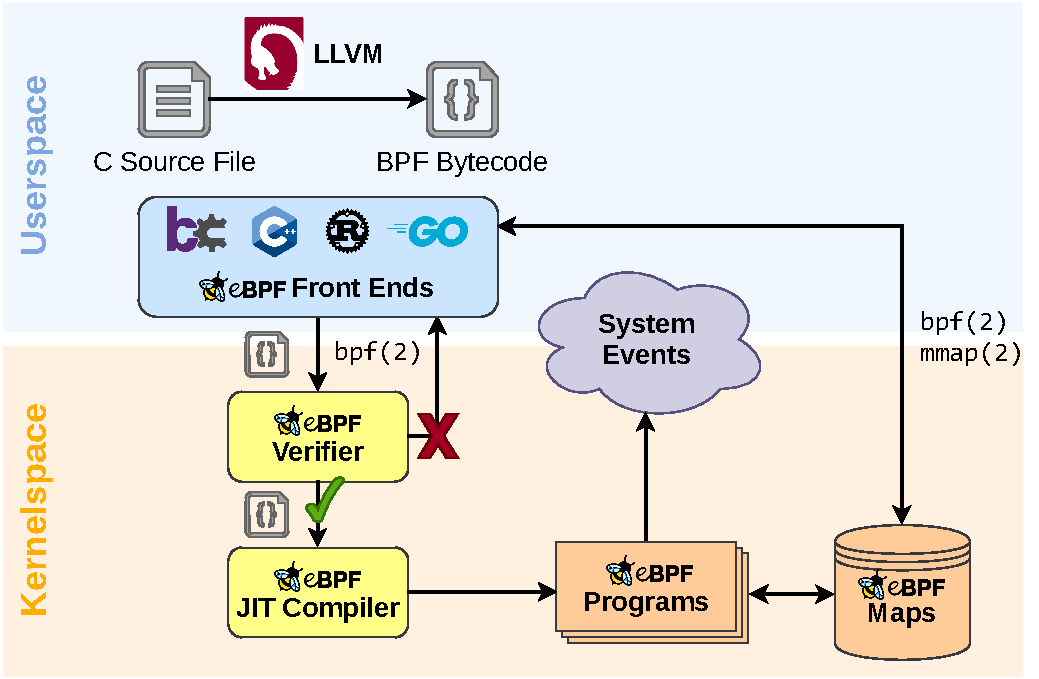
\includegraphics[height=0.85\textheight]{figs/ebpf.pdf}
\end{center}
\end{frame}

\begin{frame}[c]{Verifiable Safety}
Limited instruction set.
\begin{itemize}
    \item 11 registers (10 general purpose)
    \item 114 instructions (vs 2000+ in x86)
    \item Access to a limited set of \textbf{kernel helpers} with \texttt{call} instruction
\end{itemize}
\vfill
Restricted execution context.
\begin{itemize}
    \item 512 byte stack limit
    \item Memory access must be bounds-checked
    \item No unbounded loops
    \item No back-edges in control flow
    \item \textbf{eBPF is not Turing complete}
\end{itemize}
\end{frame}

\begin{frame}[c]{KRSI: eBPF LSM Programs}
\begin{itemize}
  \item Attach one or more eBPF programs to a given LSM hook
  \item eBPF programs can then be used to make policy decisions
  \item Works co-operatively with other LSMs (SELinux, AppArmor, etc.)
\end{itemize}
\vfill
\begin{center}
  \color{black}
  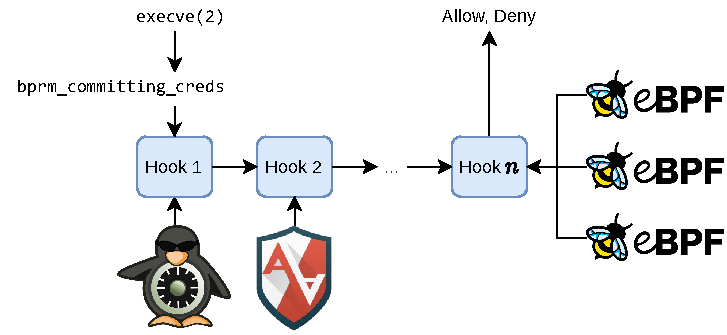
\includegraphics[height=0.5\textheight]{figs/ebpf-lsm.pdf}
\end{center}
\end{frame}

%\nocite{*}
\begin{frame}[allowframebreaks, noframenumbering, plain]
        \frametitle{References}
        \printbibliography
\end{frame}

\end{document}

% vim:syn=tex
